\documentclass{article}

\usepackage{amsmath}
\usepackage{amssymb}
\usepackage{graphicx}
\usepackage{tikz}
\usetikzlibrary{arrows}
\usepackage{verbatim}
\usepackage{sfmath}
\usepackage{psfrag}
\usepackage{here} 
\usepackage{hyperref}
\usepackage{xcolor}
\usepackage{tcolorbox}

%\renewcommand\sfdefault{phv}%               use helvetica for sans serif
\renewcommand{\familydefault}{\sfdefault}
\renewcommand{\familydefault}{cmss}

\setcounter{MaxMatrixCols}{60}

\begin{document}

\section*{Problem 2: Simulation of a car-trailer system\footnote{Adapted from \href{https://www.ensta-bretagne.fr/jaulin/automooc.pdf}{https://www.ensta-bretagne.fr/jaulin/automooc.pdf}}}



\tcbset{colframe=black,colback=white,colupper=black,fonttitle=\bfseries,nobeforeafter,center title}

Let us consider the car-trailer system represented in Figure~\ref{fig:figure} which has the following state equations:


\begin{eqnarray*}
\begin{pmatrix}
\dot{x}    \\       
\dot{y}      \\     
\dot{\theta} \\   
\dot{\theta}_r\\ 
\dot{v}           \\
\dot{\delta}   
\end{pmatrix}
=
\begin{pmatrix}
v \cos \delta \cos \theta \\
v \cos \delta \sin \theta\\
\frac{v \sin \delta}{L}\\
\frac{v \cos \delta \sin (\theta -\theta_r)}{L_r}\\
u_1\\
u_2
\end{pmatrix}.
\end{eqnarray*}
The state vector is given by
\begin{equation*}
\mathbf{x} 
=
\begin{pmatrix}
x\\
y\\
\theta\\
\theta_r\\
v\\
\delta
\end{pmatrix},
\end{equation*}
where $x, y, \theta$ corresponds to the pose of the car (in other words, its position and orientation), $\theta_r$ is the orientation of the trailer, $v$ is the speed and $\delta$ is the angle of the front wheels of the car. The
parameter $L = 3$ [m] is the distance between the two axles of the car.
The parameter $L_r = 5$ [m] represents the distance between the
attachment point and the middle of the axle of the trailer.

\begin{figure}[H]
\centerline{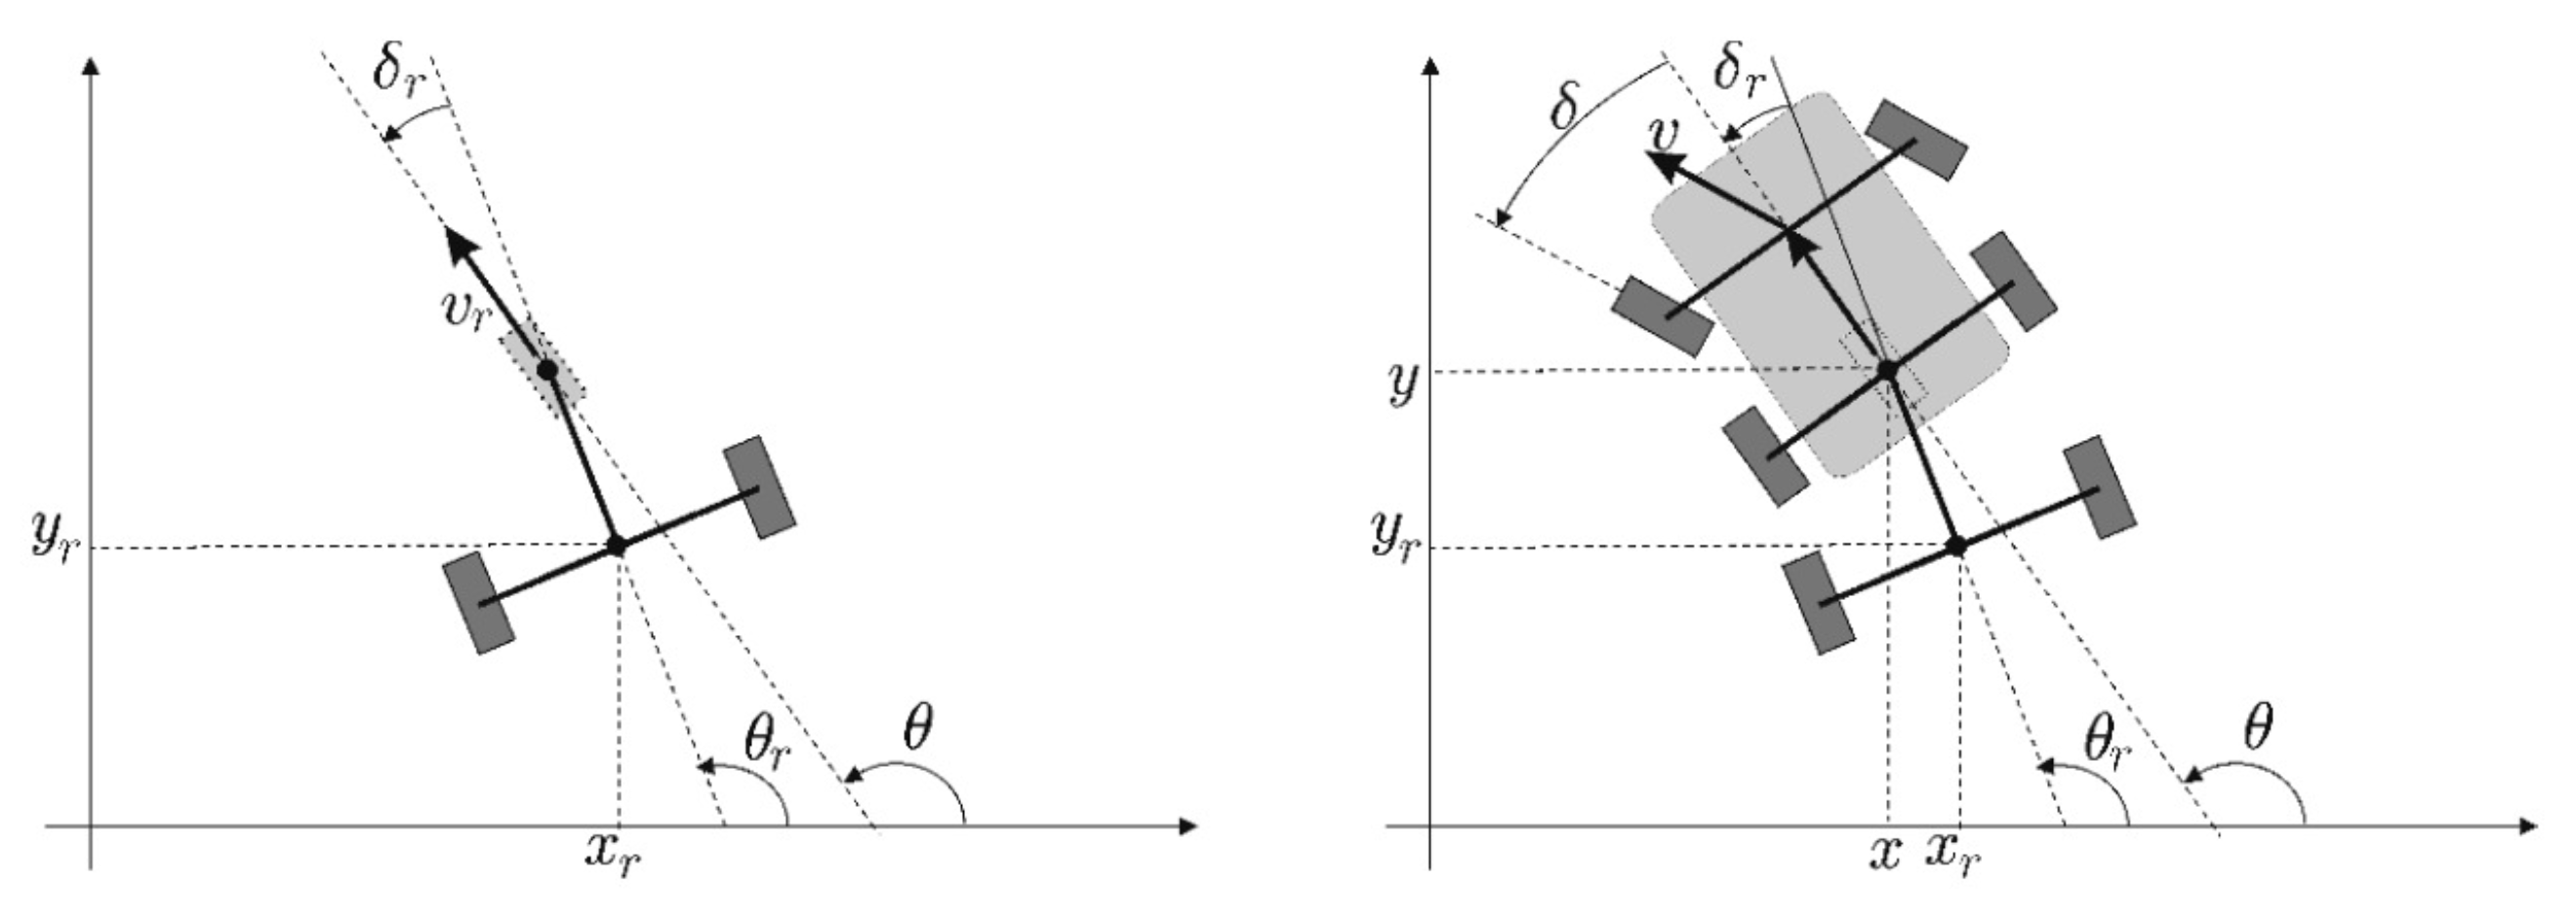
\includegraphics[width=0.99\columnwidth]{figures/car-trailer}}
\caption{The car-trailer system.}
\label{fig:figure}
\end{figure}



\begin{itemize}

\item[1)] Using homogeneous coordinates, design a function which draws a car-trailer system in a state $\mathbf{x} =
(x, y, \theta, \theta_r, v, \delta)^T$ using the sketch of the car-trailer system represented in Figure~\ref{fig:figure1} 
whose vertices in homogeneous coordinates are represented by the columns of the following matrix:

\begin{scriptsize}
 \begin{equation*}
M_{\text{trailer}} =
\begin{pmatrix}
-1 & 2  &5  &5 &2 &-1 &-1 &-1 &0  &0  &-1  &1  &0 &0 &-1 &1 &0 &0 &2 \\
-2 &-2 &0  &0 &2 &2  &-2 &-2 &-2 &-3 &-3 &-3 &-3 &3  &3 &3 &3 &2 &2\\
1 &1 &1  &1   &1   &1 &1 &1 &1 &1 &1 &1 &1 &1 &1 &1 &1 &1 &1
\end{pmatrix}.
\end{equation*}
\end{scriptsize}
The corresponding \texttt{Matlab} code is:
\begin{scriptsize}
\begin{verbatim}
M_trailer=[-1  2  5  5 2 -1 -1 -1 0  0  -1  1  0 0 -1 1 0 0 2; 
           -2 -2  0  0 2 2  -2 -2 -2 -3 -3 -3 -3 3  3 3 3 2 2;
           ones(1,19)];
\end{verbatim}                    
\end{scriptsize}                    
                    
                    
\begin{figure}[H]
\centerline{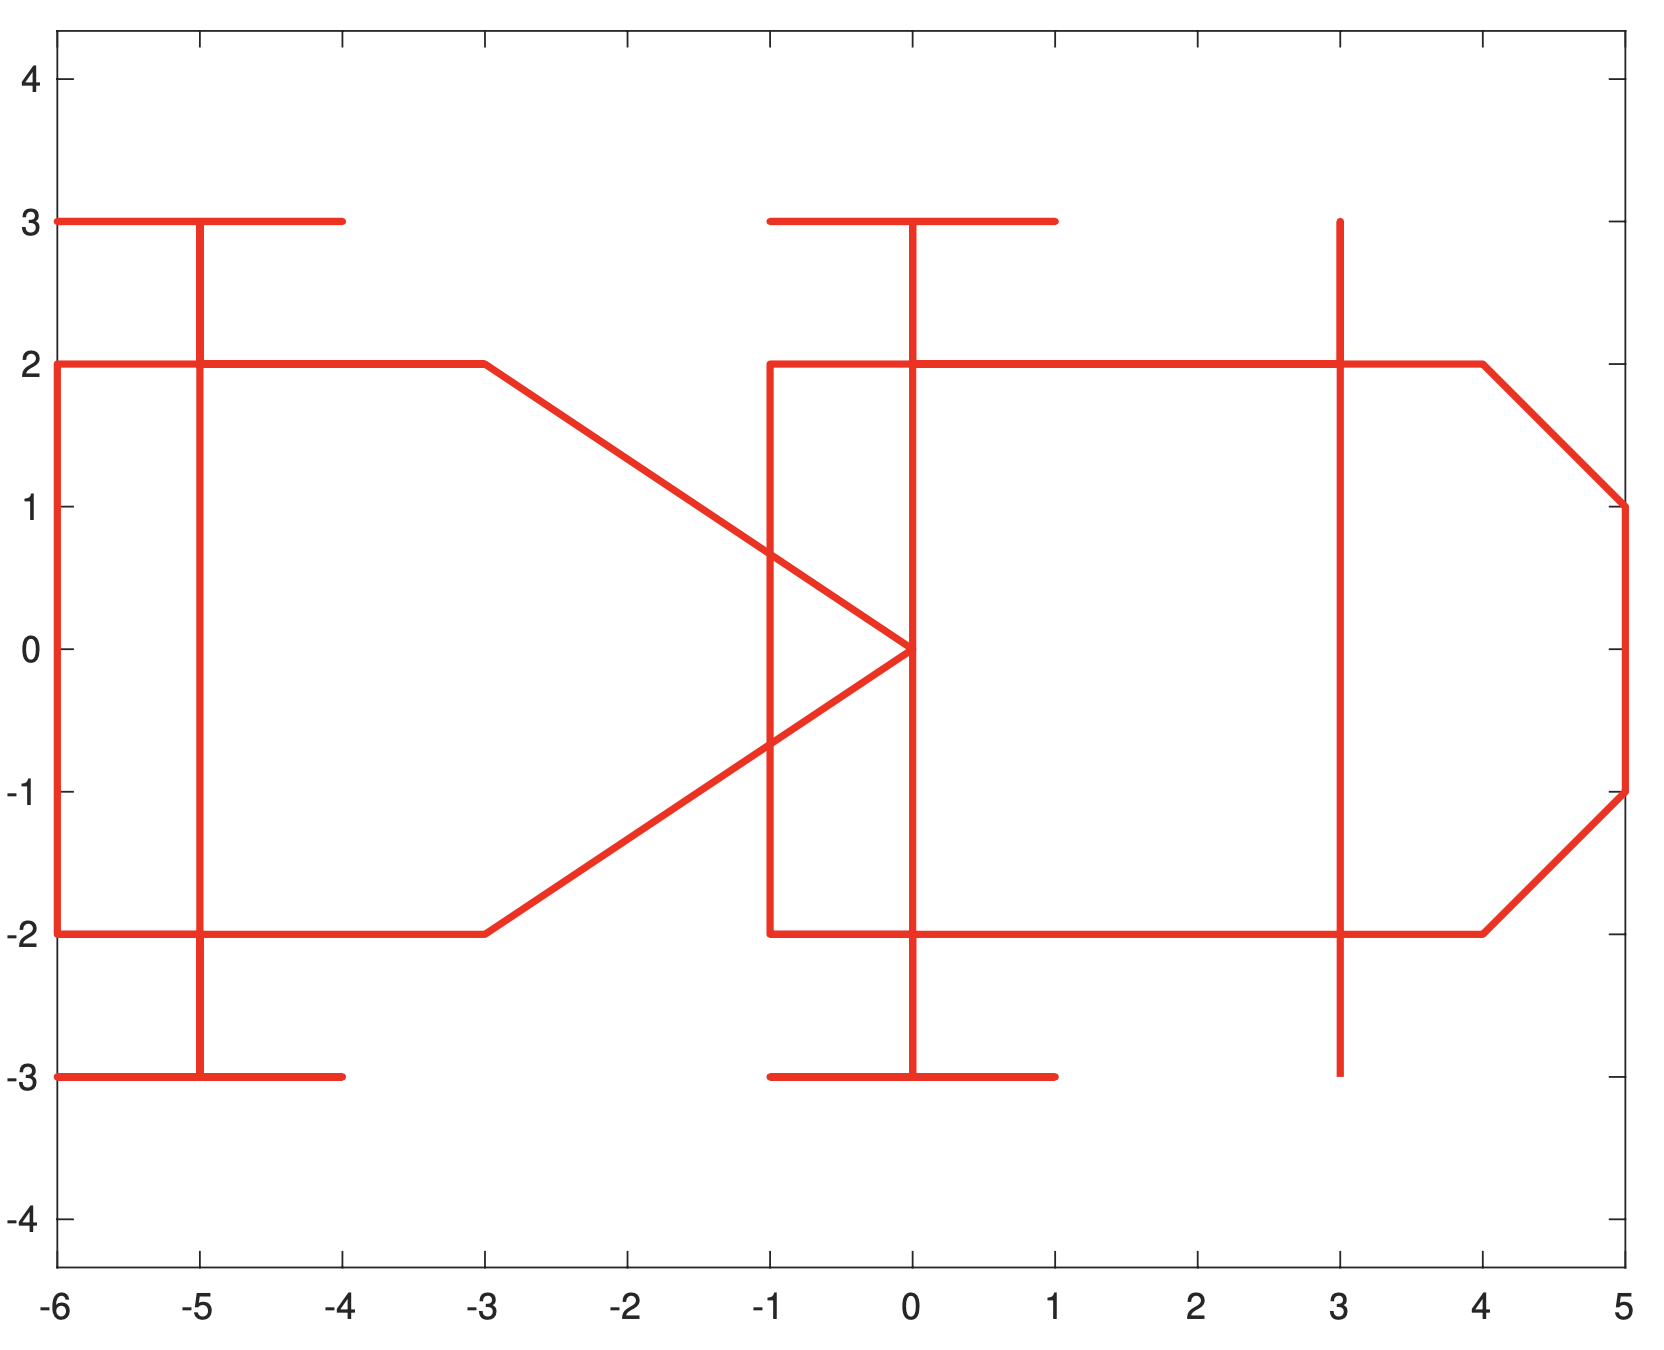
\includegraphics[width=0.99\columnwidth]{figures/chassis-trailer}}
\caption{Sketch of the car-trailer system.}
\label{fig:figure1}
\end{figure}



\item[2)] Propose a program which simulates the dynamic evolution of this car-trailer system during $5$ seconds with
Euler's method and a sampling step of $0.01 \; [\text{s}]$. Take the initial state for the car-trailer system as $\mathbf{x}(0) =
(0, 0, 0, 0, 50, 0)^T$, which means that, at time $t = 0$,

\begin{itemize}

\item
the car is centered around the origin, with a zero orientation angle, a speed of $50 \; [\text{m s}^{-1}]$ and the front wheels parallel to the axis of the car. 

\item
 the trailer has zero orientation angle. 

\end{itemize}

We assume
that the vectorial control $u(t)$ remains constant and equal to $(0, 0.05)$. Which means that the car
does not accelerate (since $u_1 = 0$) and that the steering wheel is turning at a constant speed of
$0.05 \; [\text{rad s}^{-1}]$.

\end{itemize}



\section*{Solution of Problem 2}

\begin{itemize}

{\color{gray}

\item[1)] Using homogeneous coordinates, design a function which draws a car-trailer system in a state $\mathbf{x} =
(x, y, \theta, \theta_r, v, \delta)^T$ using the sketch of the car-trailer system represented in Figure~\ref{fig:figure1} 
whose vertices in homogeneous coordinates are represented by the columns of the following matrix:

\begin{scriptsize}
 \begin{equation*}
M_{\text{trailer}} =
\begin{pmatrix}
-1 & 2  &5  &5 &2 &-1 &-1 &-1 &0  &0  &-1  &1  &0 &0 &-1 &1 &0 &0 &2 \\
-2 &-2 &0  &0 &2 &2  &-2 &-2 &-2 &-3 &-3 &-3 &-3 &3  &3 &3 &3 &2 &2\\
1 &1 &1  &1   &1   &1 &1 &1 &1 &1 &1 &1 &1 &1 &1 &1 &1 &1 &1
\end{pmatrix}.
\end{equation*}
\end{scriptsize}
The corresponding \texttt{Matlab} code is:
\begin{scriptsize}
\begin{verbatim}
M_trailer=[-1  2  5  5 2 -1 -1 -1 0  0  -1  1  0 0 -1 1 0 0 2; 
           -2 -2  0  0 2 2  -2 -2 -2 -3 -3 -3 -3 3  3 3 3 2 2;
           ones(1,19)];
\end{verbatim}                    
\end{scriptsize}                 
}                 
                    

Your solution goes here

\bigskip

\begin{tcolorbox}
[
title={File \texttt{car\_trailer\_f.m}}
]
\begin{scriptsize}
\begin{verbatim}


function  xdot  = f(x,u)
% state x = (x,y,theta,theta_r,v,delta)
% control u=(u1 u2)
L=3;
L_r=5;

px=x(1);
py=x(2);
theta=x(3);
%%%%%

%%%%%
theta_r=x(4);
v=x(5);
delta=x(6);

xdot=[v*cos(delta)*cos(theta); v*cos(delta)*sin(theta); v*sin(delta)/L; 
(v*cos(delta)*sin(theta-theta_r))/L_r; u(1); u(2)];
end



\end{verbatim}
\end{scriptsize}
\end{tcolorbox}

\bigskip

Para dibujar el trailer unido al coche debemos de modificar la representacion de estados que teniamos del coche sin trailer. Por lo tanto añadiremos theta\_r para representar el sitema coche-trailer. \\
Gracias a esta funcion obtenemos \dot{x} para poder simular la evolucion del sistema tal como especifica el siguiente apartado. 


\item[2)] 
{\color{gray}
Propose a program which simulates the dynamic evolution of this car-trailer system during $5$ seconds with
Euler's method and a sampling step of $0.01 \; [\text{s}]$. Take the initial state for the car-trailer system as $\mathbf{x}(0) =
(0, 0, 0, 0, 50, 0)^T$, which means that, at time $t = 0$,

\begin{itemize}

\item
the car is centered around the origin, with a zero orientation angle, a speed of $50 \; [\text{m s}^{-1}]$ and the front wheels parallel to the axis of the car. 

\item
 the trailer has zero orientation angle. 

\end{itemize}

We assume
that the vectorial control $u(t)$ remains constant and equal to $(0, 0.05)$. Which means that the car
does not accelerate (since $u_1 = 0$) and that the steering wheel is turning at a constant speed of
$0.05 \; [\text{rad s}^{-1}]$.
}
\end{itemize}




\bigskip





\begin{tcolorbox}
[
title={File \texttt{init.m}}
]
\begin{scriptsize}
\begin{verbatim}

close all; 
clear all; 
clc;

 
%size = get(0,'ScreenSize'); % full screen
figure%('Position',[0 0 size(3)/2 size(4)/2]);
hold
% set(gca,'FontSize',12);
xmin=-10;
xmax=100;
ymin=-10;
ymax=100;

axis([xmin xmax ymin ymax]); 
axis ('square');


\end{verbatim}
\end{scriptsize}
\end{tcolorbox}


\begin{tcolorbox}
[
title={File \texttt{car\_trailer\_main.m}}
]
\begin{scriptsize}
\begin{verbatim}


init;

%For this system, the state is x =(x,y,theta,theta_r,v,delta)

x=[0;0;0;0;50;0]; % Initial state

dt=0.01;

frame_counter=0;

car_trailer_draw(x); 
plot(x(1), x(2),'red.','MarkerSize',12)

for t=0:dt:5
    
    u1=0;
    u2=0.05;
    u=[u1;u2];
    x=x+car_trailer_f(x,u)*dt; % Euler
    
    pause(dt);
    
    frame_counter =frame_counter+1;
    
    % Frame sampling
    if frame_counter == 30
       car_trailer_draw(x); 
       plot(x(1), x(2),'red.','MarkerSize',12)
       frame_counter =0;
    end
end;




\end{verbatim}
\end{scriptsize}
\end{tcolorbox}

\begin{tcolorbox}
[
title={File \texttt{car\_trailer\_draw.m}}
]
\begin{scriptsize}
\begin{verbatim}


% For this system, the state is x =(x,y,theta,v,delta)
% The v state variable, since it is a speed, it is not used in this 
% graphical representation

function car_trailer_draw(x)

   % Extraction of the state variables
   px = x(1);
   py = x(2);
   theta = x(3);
   theta_r = x(4);
   v = x(5);
   delta = x(6);
  
   % Model of the chassis of the car without front wheels (in homogeneous coordinates)
   M_chassis=[-1  4 5  5 4 -1 -1 -1 0  0  -1  1  0 0 -1 1 0 0 3 3 3; 
              -2 -2 -1 1 2 2  -2 -2 -2 -3 -3 -3 -3 3  3 3 3 2 2 3 -3;
              ones(1,21)];
  
   % Model of a front wheel (in homogeneous coordinates)
   M_wheel=[-1 1;
            0 0;
            1 1]; 
   
   
   % Translation and rotation of the whole car (chassis and front wheels) 
   % with respect to the fixed frame
   TR_px_py_theta = [cos(theta),-sin(theta), px;
                 sin(theta),cos(theta), py;
                 0 0 1]; 
   
   % Chassis of the car translated and rotated
   M_chassis_transformed=TR_px_py_theta * M_chassis;   
   
   % Translation and rotation matrix for the right wheel 
   % with respect to the chassis frame 
   TR_right_wheel_delta = [cos(delta),-sin(delta), 3;
                           sin(delta),cos(delta), 3 ;
                           0 0 1]; 
   
   % Translation and rotation matrix for the left wheel 
   % with respect to the chassis frame
   TR_left_wheel_delta = [cos(delta),-sin(delta), 3;
                          sin(delta),cos(delta), -3;
                          0 0 1]; 
   
   % Right front wheel translated and rotated (first with respect to the chassis frame 
   % and then with respect to the fixed frame)
   M_right_wheel_transformed = TR_px_py_theta*TR_right_wheel_delta*M_wheel; 
   
   % Left front wheel wheel translated and rotated 
   % (first with respect to the chassis frame 
   % and then with respect to the fixed frame)
   M_left_Wheel_transformed = TR_px_py_theta*TR_left_wheel_delta*M_wheel; 

\end{verbatim}
\end{scriptsize}
\end{tcolorbox}

\bigskip

\begin{tcolorbox}
[
title={File \texttt{car\_trailer\_draw.m}}
]
\begin{scriptsize}
\begin{verbatim}

   %-----------------------------------------------------------------------
   
   % Model of the trailer (in homogeneous coordinates)     
   M_trailer = [-1  2  5  5 2 -1 -1 -1 0  0  -1  1  0 0 -1 1 0 0 2 ; 
              -2 -2  0  0 2 2  -2 -2 -2 -3 -3 -3 -3 3  3 3 3 2 2 ;
              ones(1,19)];
   
   T_trailer = [1 0 -5;0 1 0;0 0 1];

   TR_trailer_px_py_theta = [cos(theta_r),-sin(theta_r), px;
                             sin(theta_r),cos(theta_r),  py;
                             0 0 1]; 

   M_trailer_transformed = TR_trailer_px_py_theta*T_trailer*M_trailer;
   
   %-----------------------------------------------------------------------
   
 
   plot(M_chassis_transformed(1,:), M_chassis_transformed(2,:), 'red', 'LineWidth', 1);
               
   plot(M_right_wheel_transformed(1,:), M_right_wheel_transformed(2,:), 
   	'black', 'LineWidth', 1);
   	
   plot(M_left_Wheel_transformed(1,:), M_left_Wheel_transformed(2,:),
   	 'black', 'LineWidth',1);  
    
   plot(M_trailer_transformed(1,:), M_trailer_transformed(2,:), 'blue', 'LineWidth', 1);            

end

\end{verbatim}
\end{scriptsize}
\end{tcolorbox}

\bigskip

Mediante el empleo de estos 4 ficheros teniendo en cuenta el mostrado en el apartado 1, podemos recrear la simulación del sistema de coche y trailer, siendo el coche representado en color rojo y el trailer en azul para que sea mas facil diferenciarlos. En el fichero init.m, inicializamos los ejes; el fichero car\_trailer\_draw.m realizamos las traslaciones y las rotaciones necesarias de las ruedas frontales del coche y del trailer, ambos con respecto al chasis del coche; y por ultimo en el fichero car\_trailer\_main.m, aplicamos el metodo de Euler para realizar la simulacion del sistema durante 5 segundos tal como se especifica.\\
A continuacion se muestra el resultado final de la simulacion del sistema: 


\begin{figure}[H]
\centerline{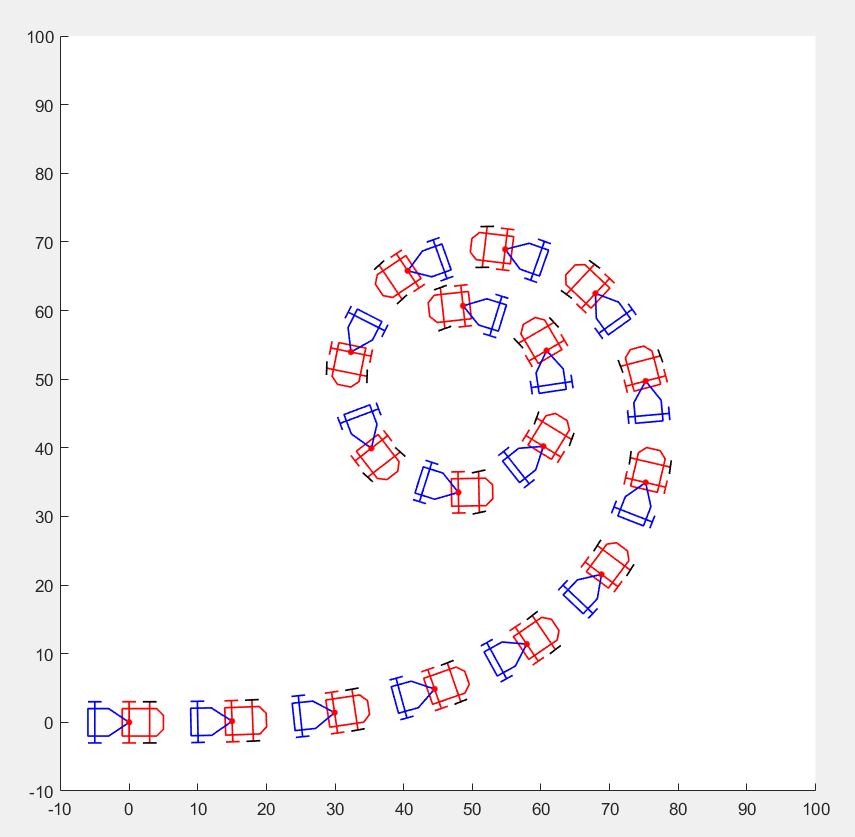
\includegraphics{figures/simulation}}
\caption{Simulation of the car-trailer system.}
\label{fig:figure2}
\end{figure}


\end{document}
